\section{Problemidentifikation}
\subsection{Idegenerering}
\subsubsection{Mindmap}
Vi har valgt at lave et mindmap, da dette er en effektiv måde at generere ideer på, og få et overblik over hvilke emner der er relevante at beskæftige sig med.
\begin{figure}[H]
    \centering
    \fbox{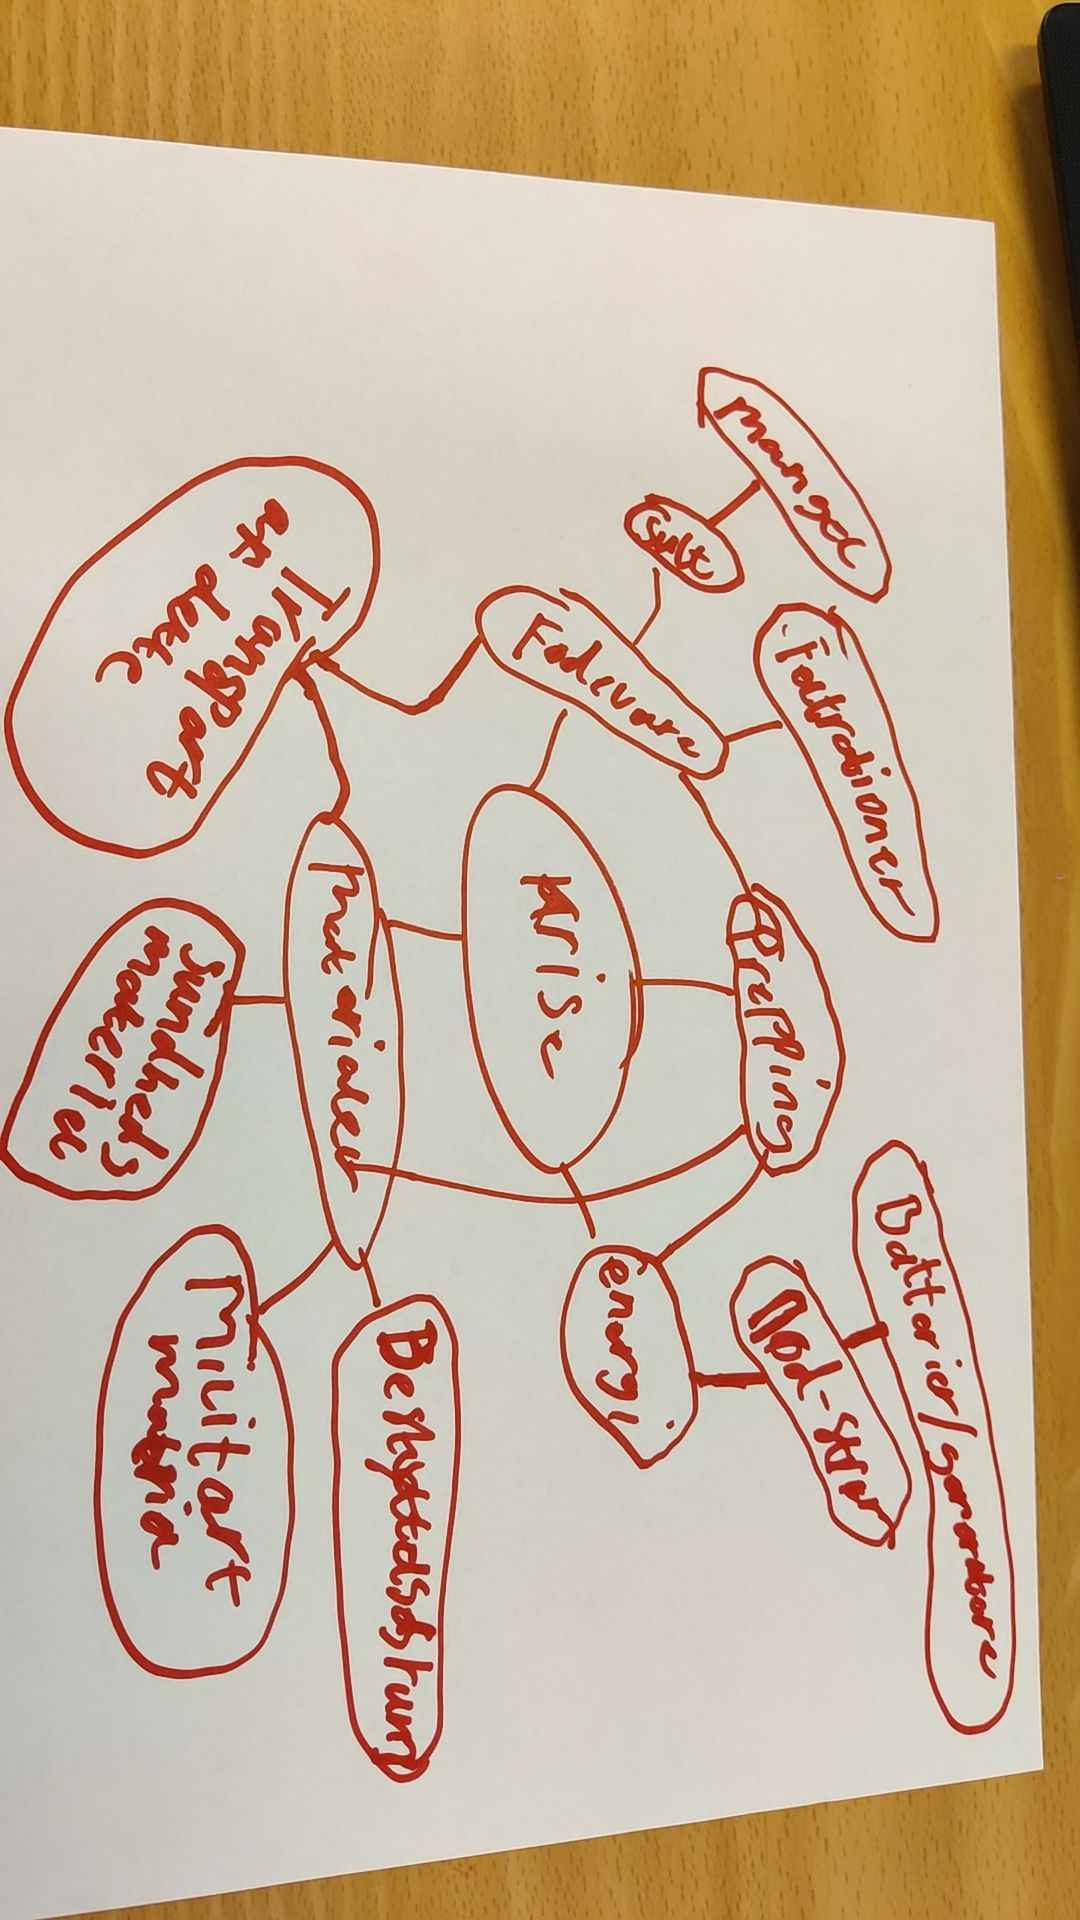
\includegraphics[scale=0.25, angle=90]{assets/section_3/mindmap.jpg}}
    \caption{Viser vores mindmap}
\end{figure}

\subsubsection{Lyskurven}
Lyskurven er en metode, man kan bruge til at sortere ideerne i forhold til hvilke der er mest relevante.
----- Bla bla waffel mere on lyskurvediagrammet -----

\begin{table}[H]
    \centering
    \begin{tabular}{|c|c|c|}
        \hline
        Fødevarer & \textbf{Grøn} \\
        \hline
        Beskyttelsesrum & \textbf{Gul} \\
        \hline
        Nødstrøm & \textbf{Rød} \\
        \hline
    \end{tabular}
    \caption{Viser et meget abstrakt lyskurvediagram i form af en tabel; det vi anvendte}
\end{table}

\subsubsection{Identificering af nøgleproblem}
Ved identifikation af et nøgleproblem, kan man sortere i sine ideer ved at opstille følgende spørgsmål:
\begin{enumerate}
    \item Hvorfor er det her interessant?
    \item Hvem er det interessant for?
    \item Er det noget, vi laver for vores egen fornøjelses skyld?
    \item Er det noget, som en bestemt gruppe i samfundet kan have gavn af, eller er det noget, der er til gavn for alle?
\end{enumerate}
** Spørsmålene som vi her gør brug af er hentet fra systimebogen\footnote{\href{https://projektarbejdet.systime.dk/?id=271}{Projektarbejdet}}

Besvarelsen på disse spørgsmål ser således ud:
\begin{enumerate}
    \item Krisehåndtering er et interessant emne, da det har en stor betydning for alle i samfundet.
    \item Det er relavant for alle.
    \item Nej, ideen med produktet er at kunne hjælpe almindelige mennesker med at håndtere kriser, mindre som store.
    \item Produktet skulle kunne gavne alle, som kunne stå i en krisesituation.
\end{enumerate}

Vi kan nu se, at det mest interessante emne er krisehåndtering, da det har en så stor relavans for grupper i samfundet, og det er noget som vi ser der er behov for.